\section{Experiment 1: Feature Extraction}
In this section we extract the features for CIFAR10 and CIFAR100 with the method described in Section 3. With early stop method, the final test accuracy of CIFAR10 is 0.9241, for CIFAR100 the accuracy is 0.7266. The training history is shown in appendix.

\begin{figure}[H]
\centering  
\subfigure[CIFAR10]{
\label{Fig.sub.a1}
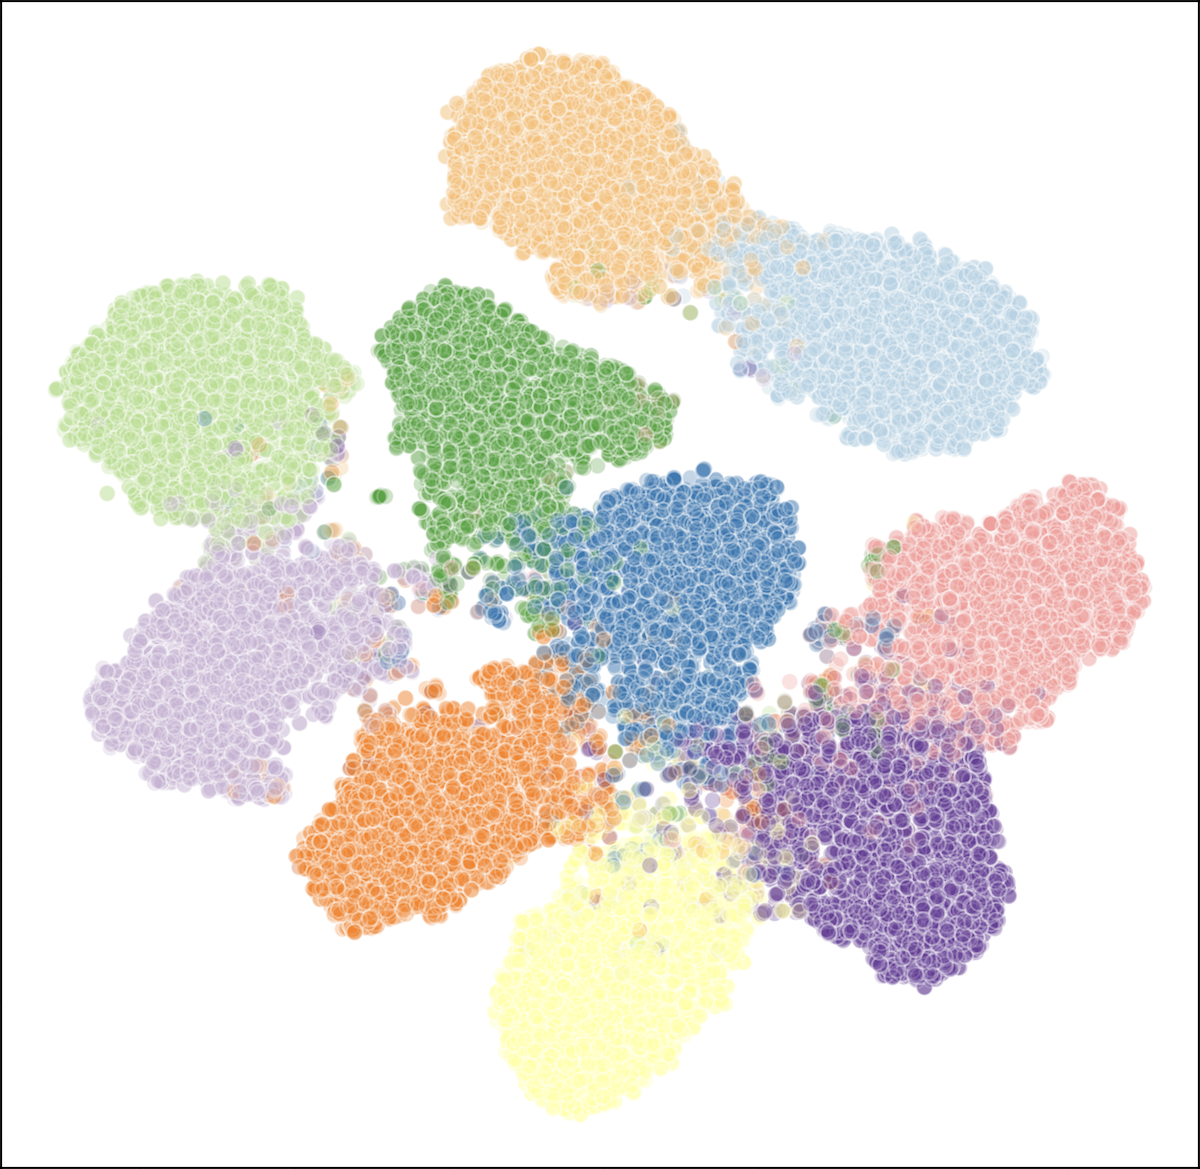
\includegraphics[width=0.45\textwidth]{src/cifar10-tsne.png}}
\subfigure[CIFAR100]{
\label{Fig.sub.a2}
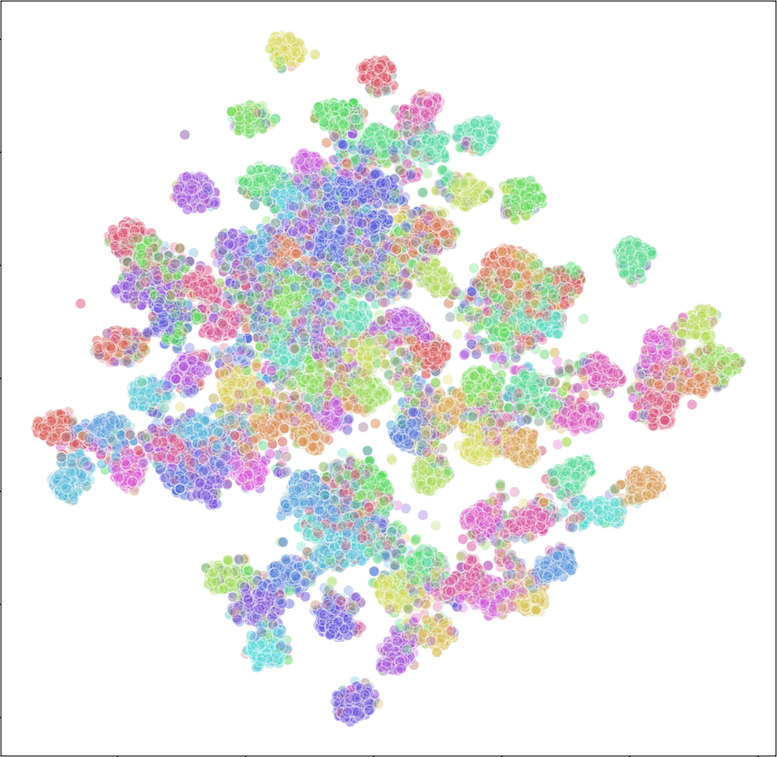
\includegraphics[width=0.45\textwidth]{src/cifar100-tsne.png}}
\caption{Extracted features visualisation with t-SNE algorithm}
\label{Fig.tsne}
\end{figure}

\begin{figure}[H]
\centering  
\subfigure[CIFAR10]{
\label{Fig.sub.a1}
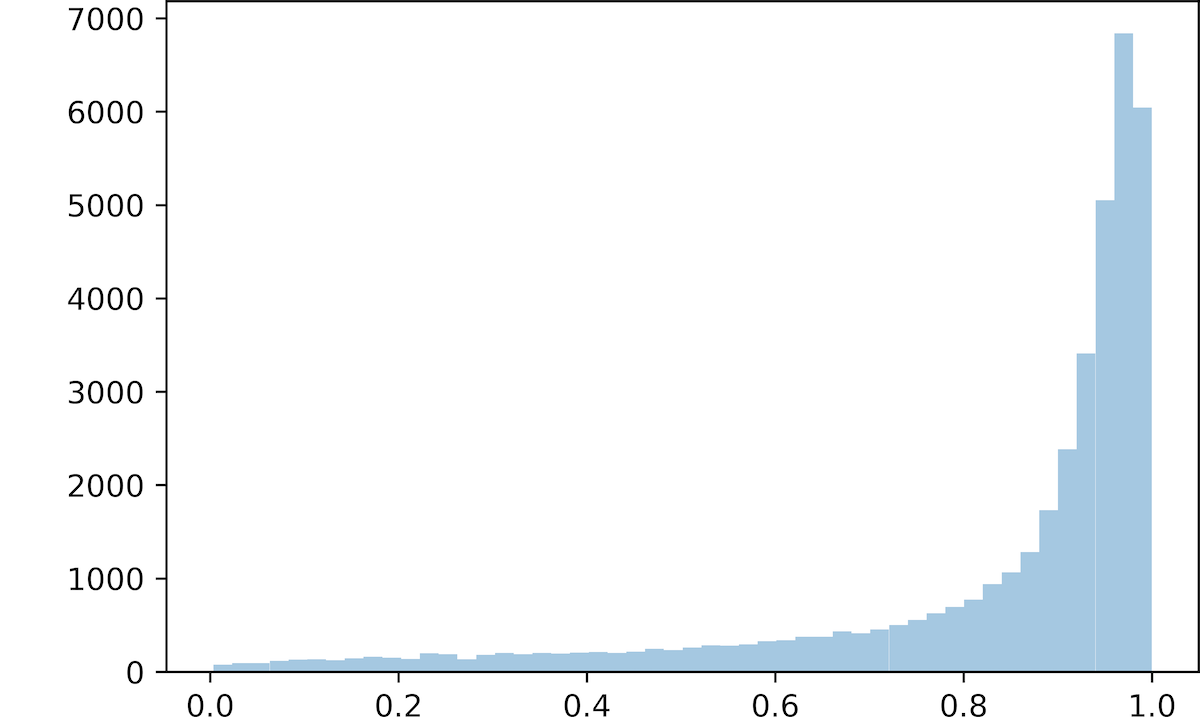
\includegraphics[width=0.45\textwidth]{src/cl_score_cifar10.png}}
\subfigure[CIFAR100]{
\label{Fig.sub.a2}
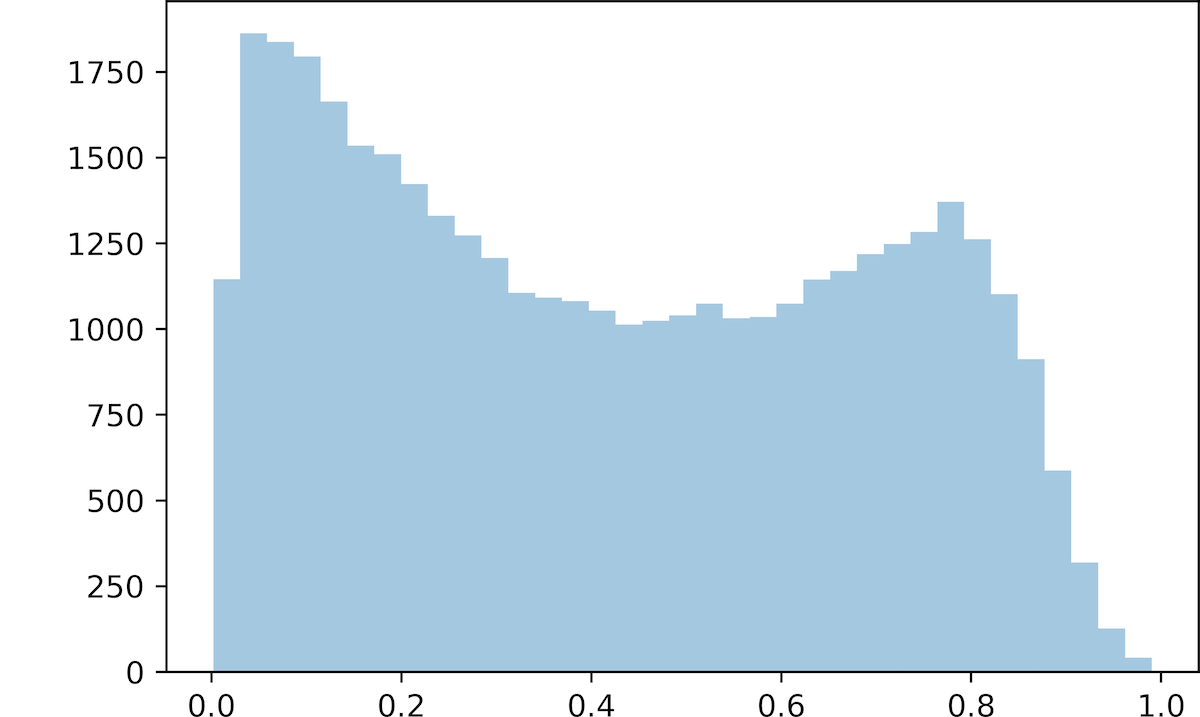
\includegraphics[width=0.45\textwidth]{src/cl_score_cifar100.png}}
\caption{Score distribution}
\label{Fig.clscores}
\end{figure}

\section{Experiment 2: Intrinsic Behaviour}
In this section, we use CIFAR10 to show the intrinsic behaviour of each data reduction algorithm described in Section 3. First we visualise the compressed cifar10 training features with the t-SNE algorithm, which projects the features down to 2 dimensional and maintains the relative distance between samples.

\subsection{Tuneable Parameters and Sample Preference}
For POP, we can tune the difference tolerance. For EGDIS, we can tune the k of the k-NN classifier. For CL, we can tune the number of samples selected. For WCL, we can tune the difficulty sample portion.

\begin{figure}[H]
\centering  
\subfigure[T=1, 8701 samples]{
\label{Fig.sub.a1}
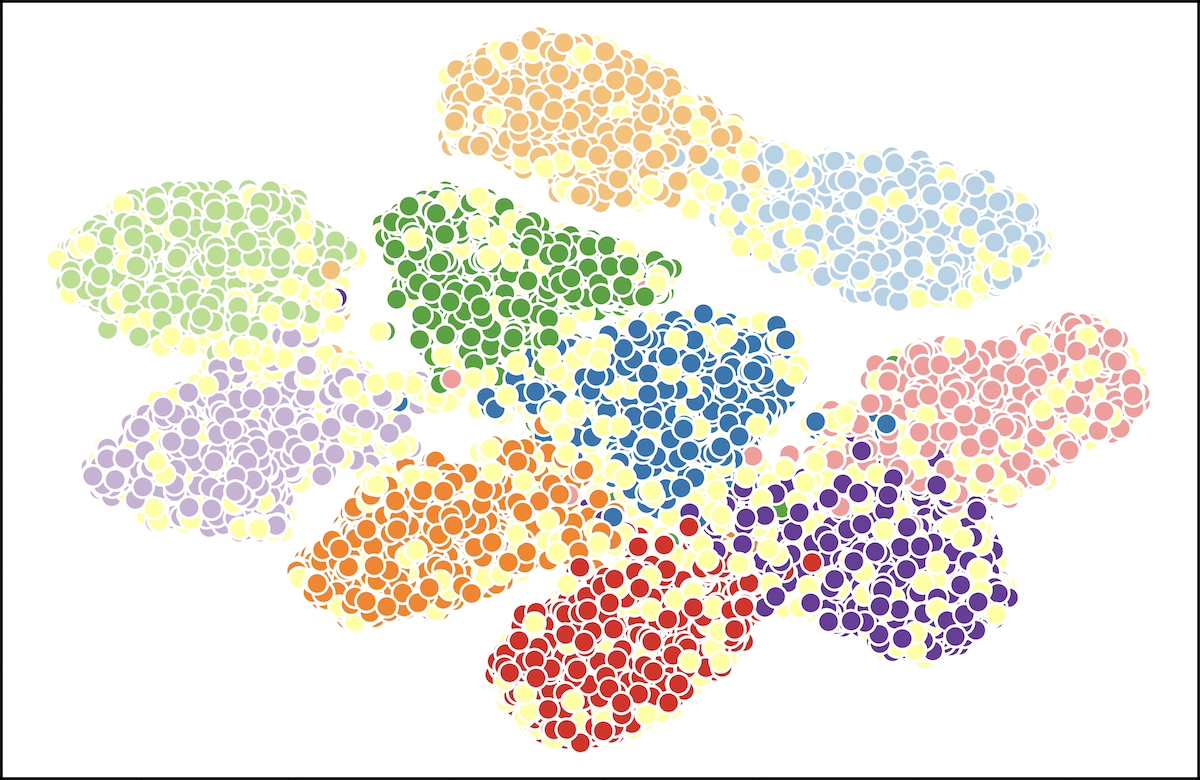
\includegraphics[width=0.32\textwidth]{src/pop-cifar10-1.png}}
\subfigure[T=0.5, 14111 samples]{
\label{Fig.sub.a2}
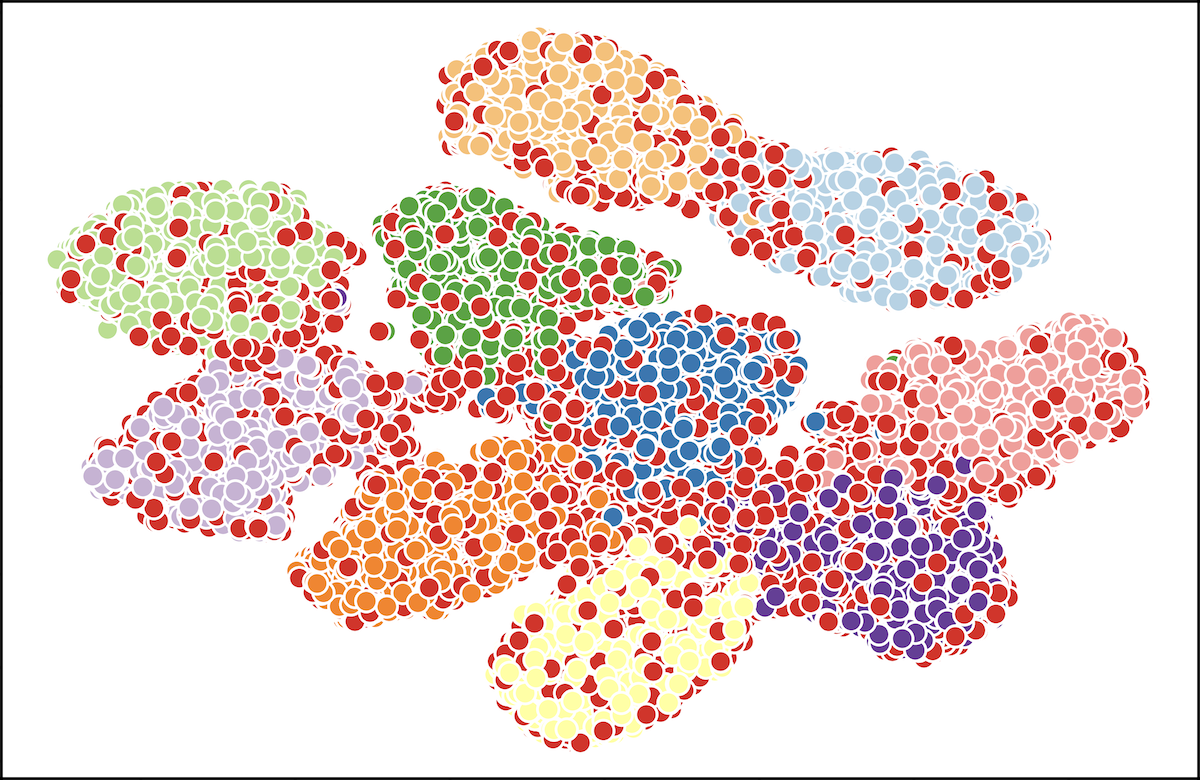
\includegraphics[width=0.32\textwidth]{src/pop-cifar10-5.png}}
\subfigure[T=0.1, 31966 samples]{
\label{Fig.sub.a1}
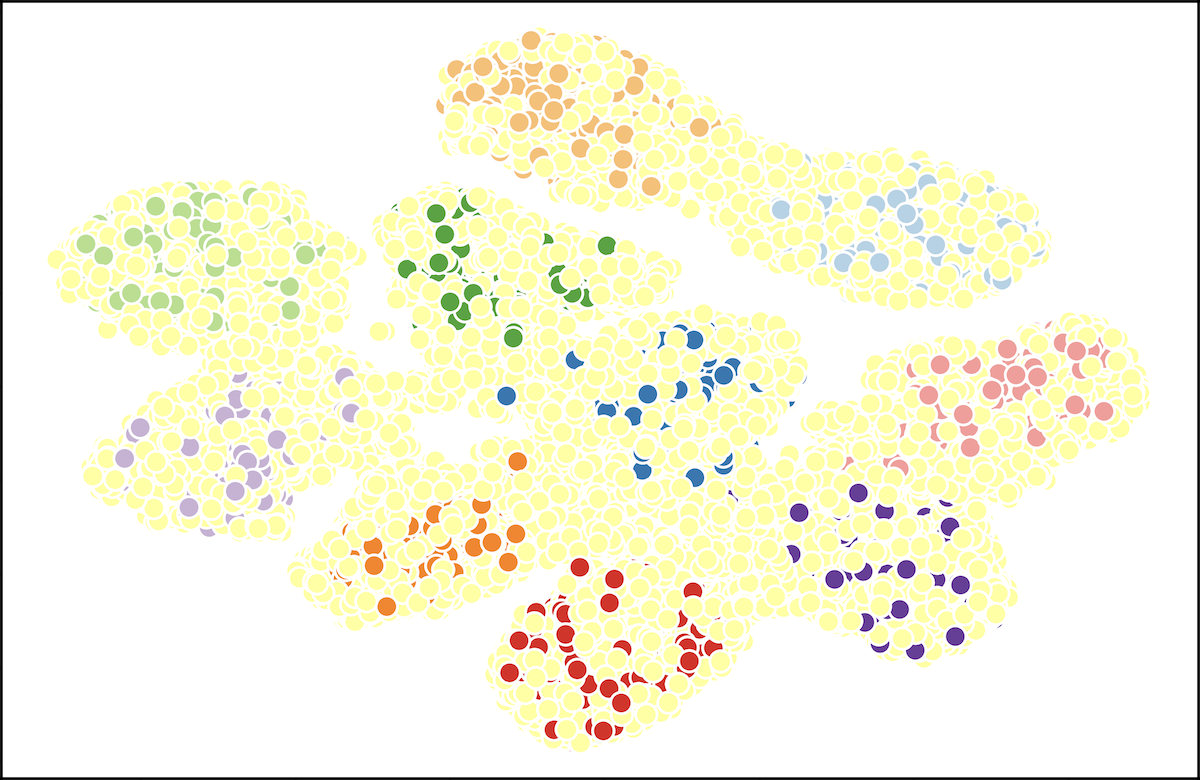
\includegraphics[width=0.32\textwidth]{src/pop-cifar10-01.png}}
\caption{POP tune threshold}
\label{Fig.popcifar10}
\end{figure}

\begin{figure}[H]
\centering  
\subfigure[k=7, 3313 samples]{
\label{Fig.sub.a1}
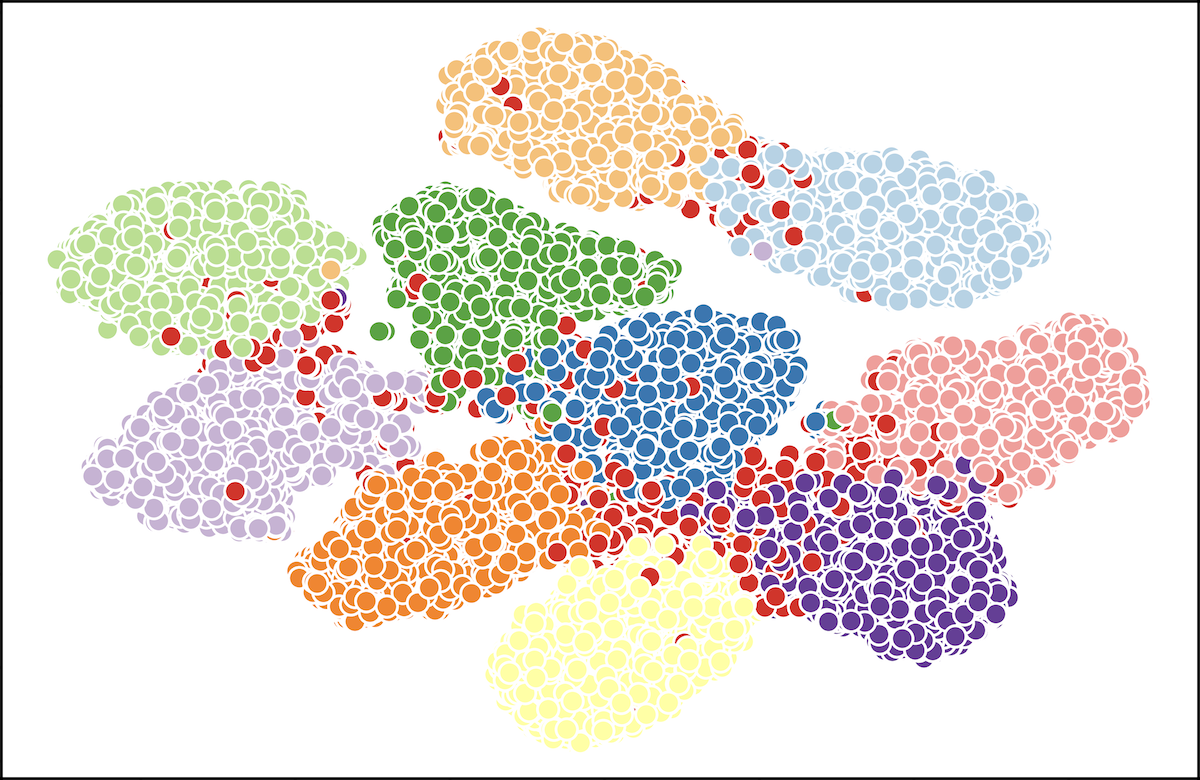
\includegraphics[width=0.32\textwidth]{src/egdis-cifar10-8.png}}
\subfigure[k=5, 4034 samples]{
\label{Fig.sub.a2}
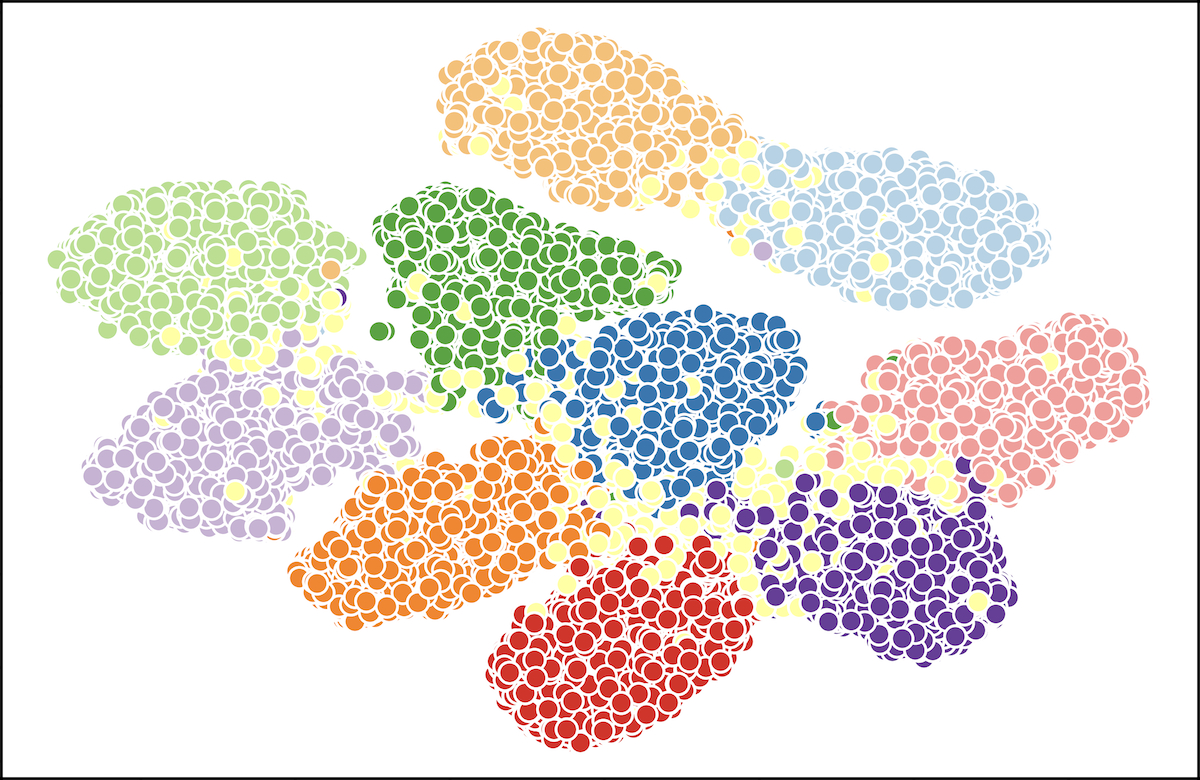
\includegraphics[width=0.32\textwidth]{src/egdis-cifar10-6.png}}
\subfigure[k=3, 5966 samples]{
\label{Fig.sub.a1}
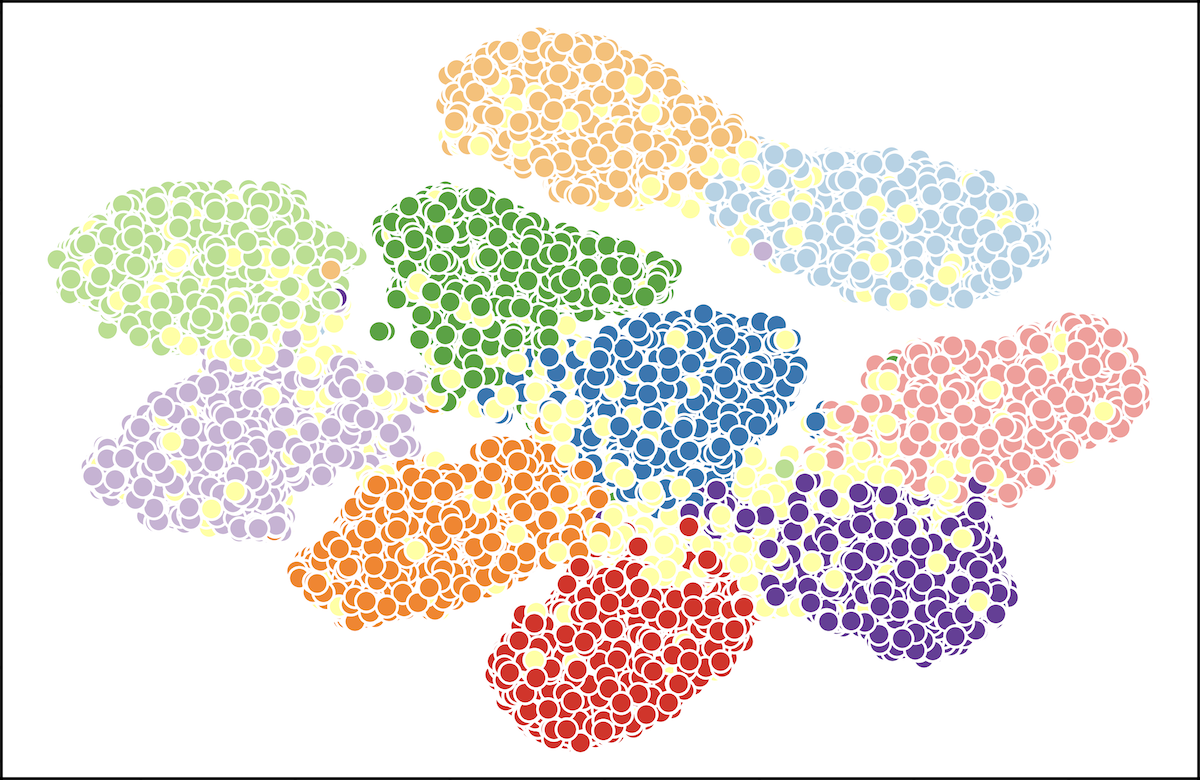
\includegraphics[width=0.32\textwidth]{src/egdis-cifar10-4.png}}
\caption{EGDIS tune kNN}
\label{Fig.egdiscifar10}
\end{figure}




\begin{figure}[H]
\centering  
\subfigure[P=10\%, 4000 samples]{
\label{Fig.sub.a1}
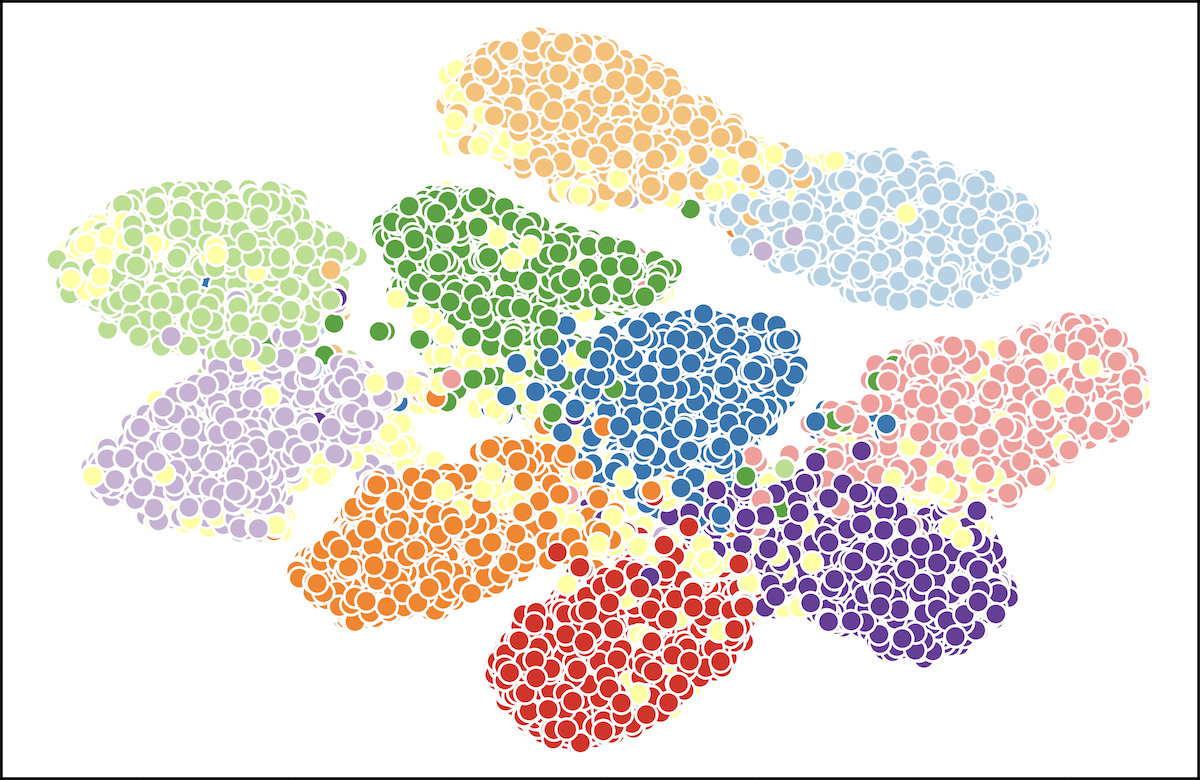
\includegraphics[width=0.32\textwidth]{src/cl-cifar10-1.png}}
\subfigure[P=30\%, 12000 samples]{
\label{Fig.sub.a2}
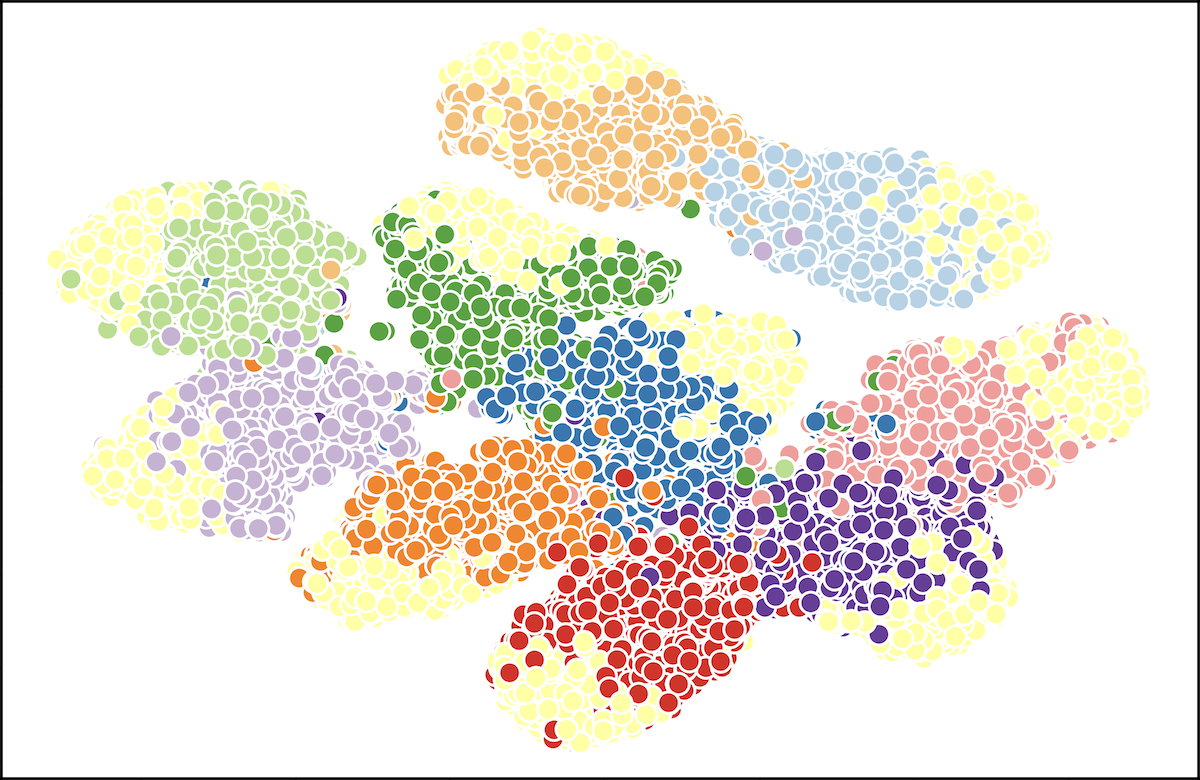
\includegraphics[width=0.32\textwidth]{src/cl-cifar10-3.png}}
\subfigure[P=50\%, 20000 samples]{
\label{Fig.sub.a1}
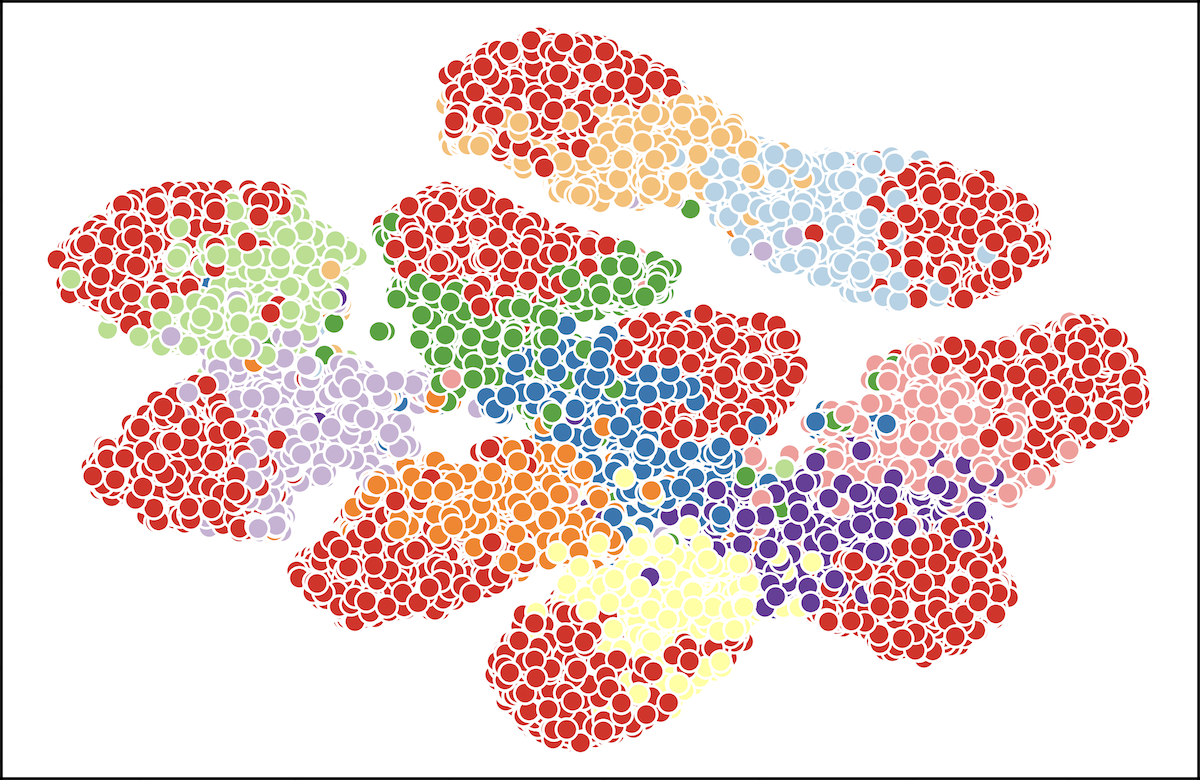
\includegraphics[width=0.32\textwidth]{src/cl-cifar10-5.png}}
\caption{CL tune selection percentage}
\label{Fig.clcifar10}
\end{figure}

WCL which takes the sample within each class based on the sample score. Although most samples are selected from the high score region, there are some sample selected from the low score region. The problem is that for relatively easy dataset like CIFAR10, the behaviour is close to random selection because most samples have a score higher than 0.8. The score distribution is shown below.

\begin{figure}[H]
\centering  
\subfigure[CIFAR10]{
\label{Fig.sub.a1}
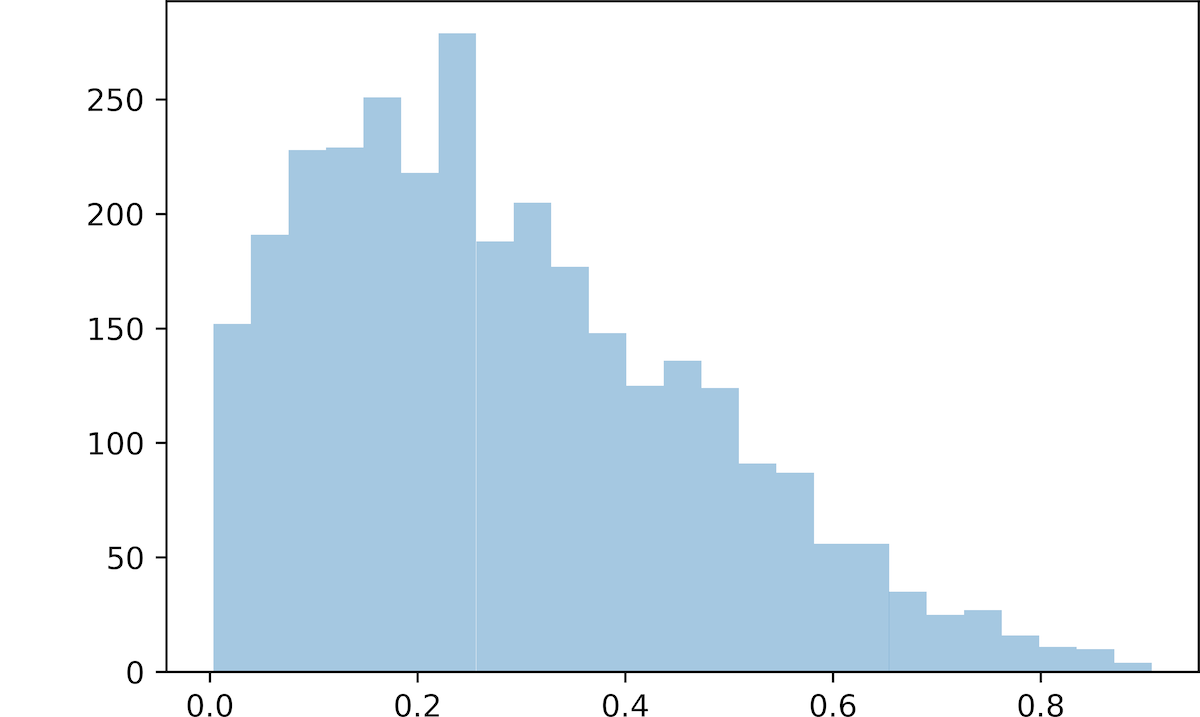
\includegraphics[width=0.45\textwidth]{src/boundarydis-cifar10-dis.png}}
\subfigure[CIFAR100]{
\label{Fig.sub.a2}
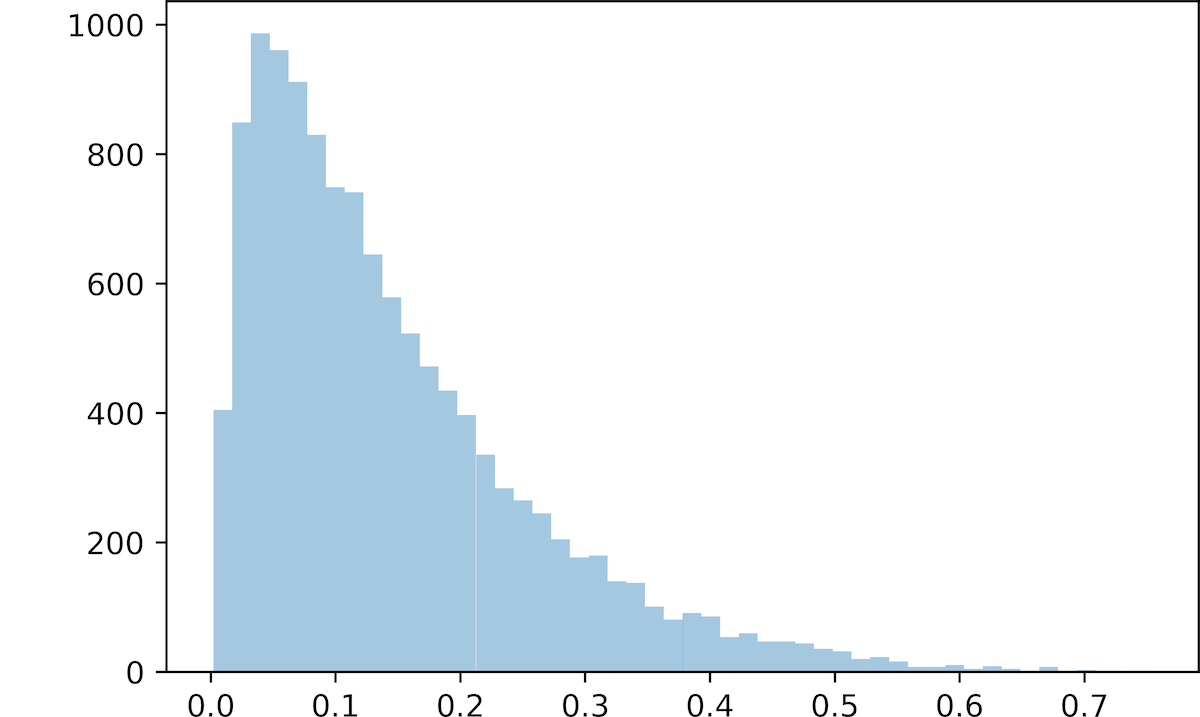
\includegraphics[width=0.45\textwidth]{src/boundarydis-cifar100-dis.png}}
\caption{EGDIS boundary score distribution}
\label{Fig.egdisboscores}
\end{figure}

\begin{figure}[H]
\centering  
\subfigure[P=10\%, 4000 samples]{
\label{Fig.sub.a1}
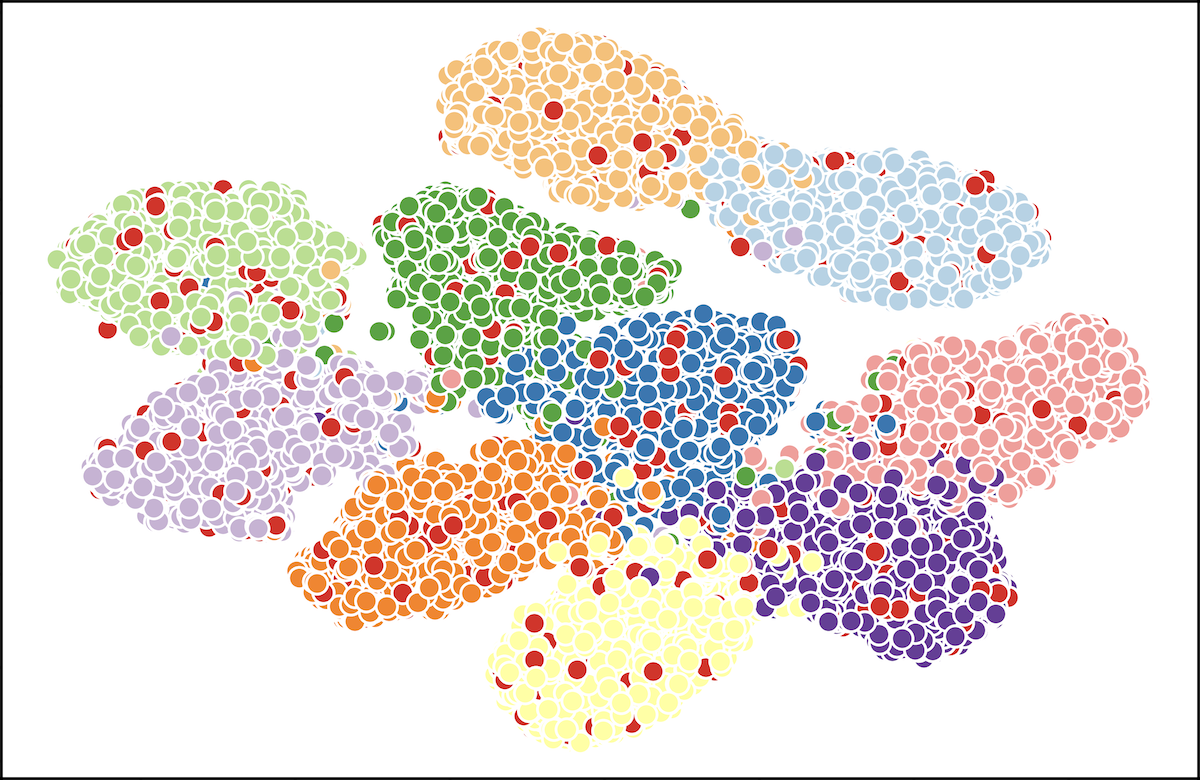
\includegraphics[width=0.32\textwidth]{src/wcl-cifar10-1.png}}
\subfigure[P=30\%, 12000 samples]{
\label{Fig.sub.a2}
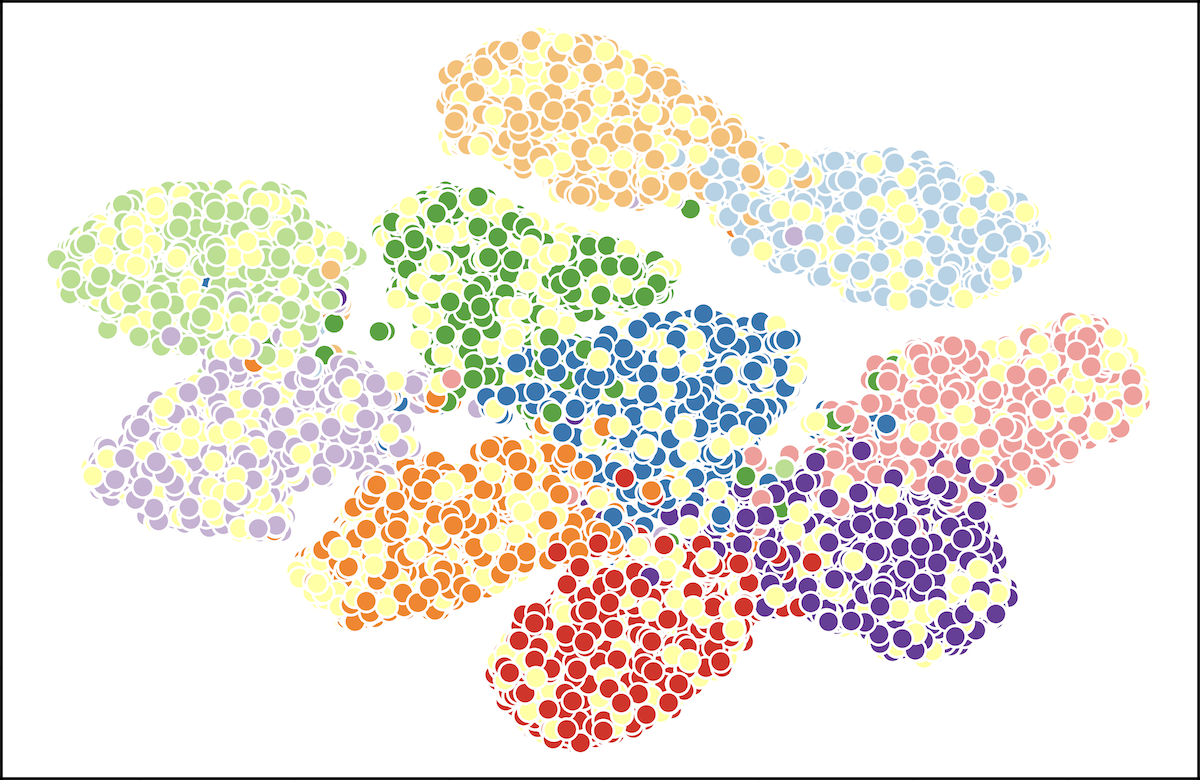
\includegraphics[width=0.32\textwidth]{src/wcl-cifar10-3.png}}
\subfigure[P=50\%, 20000 samples]{
\label{Fig.sub.a1}
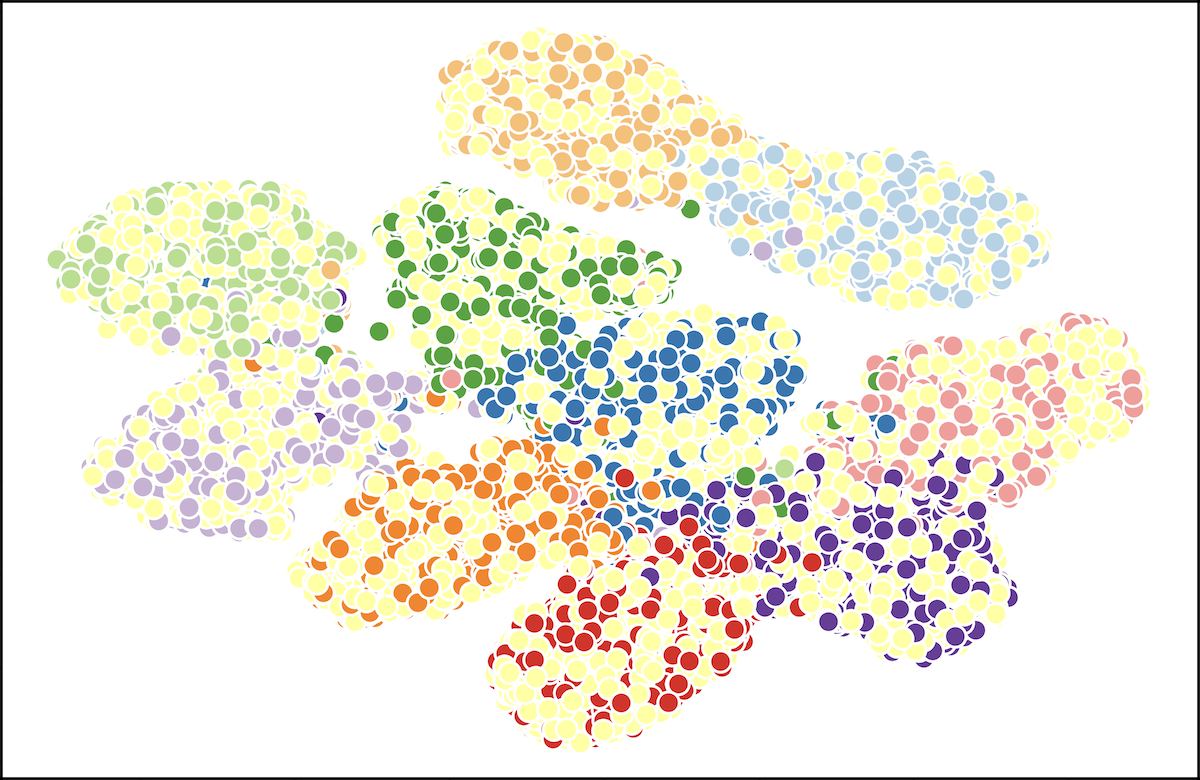
\includegraphics[width=0.32\textwidth]{src/wcl-cifar10-5.png}}

\subfigure[P=10\%, 4000 samples]{
\label{Fig.sub.a1}
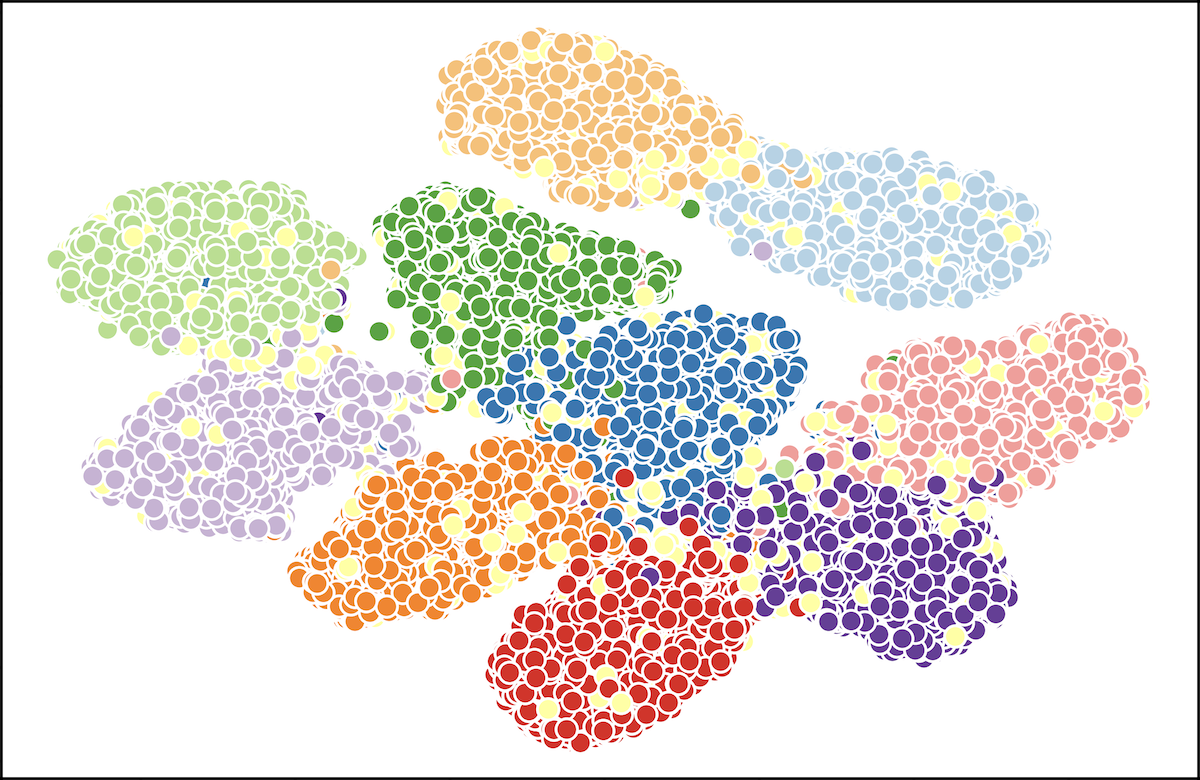
\includegraphics[width=0.32\textwidth]{src/wcl2-cifar10-1.png}}
\subfigure[P=30\%, 12000 samples]{
\label{Fig.sub.a2}
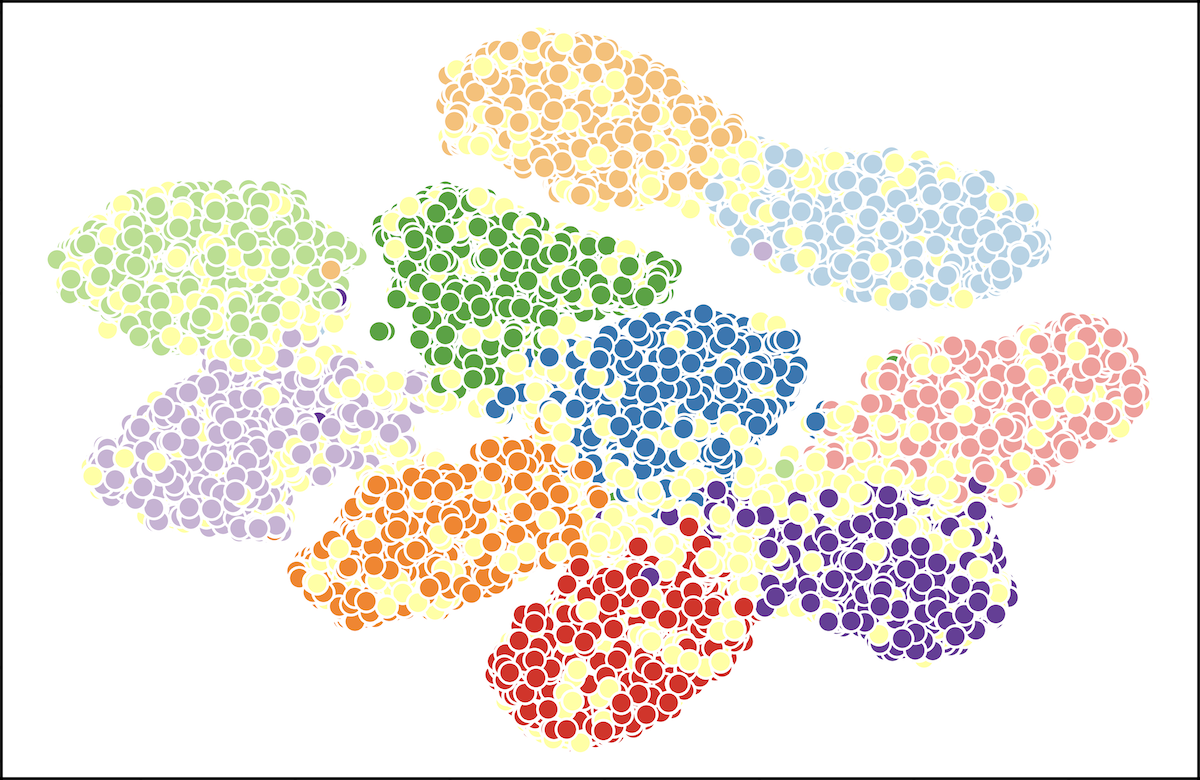
\includegraphics[width=0.32\textwidth]{src/wcl2-cifar10-3.png}}
\subfigure[P=50\%, 20000 samples]{
\label{Fig.sub.a1}
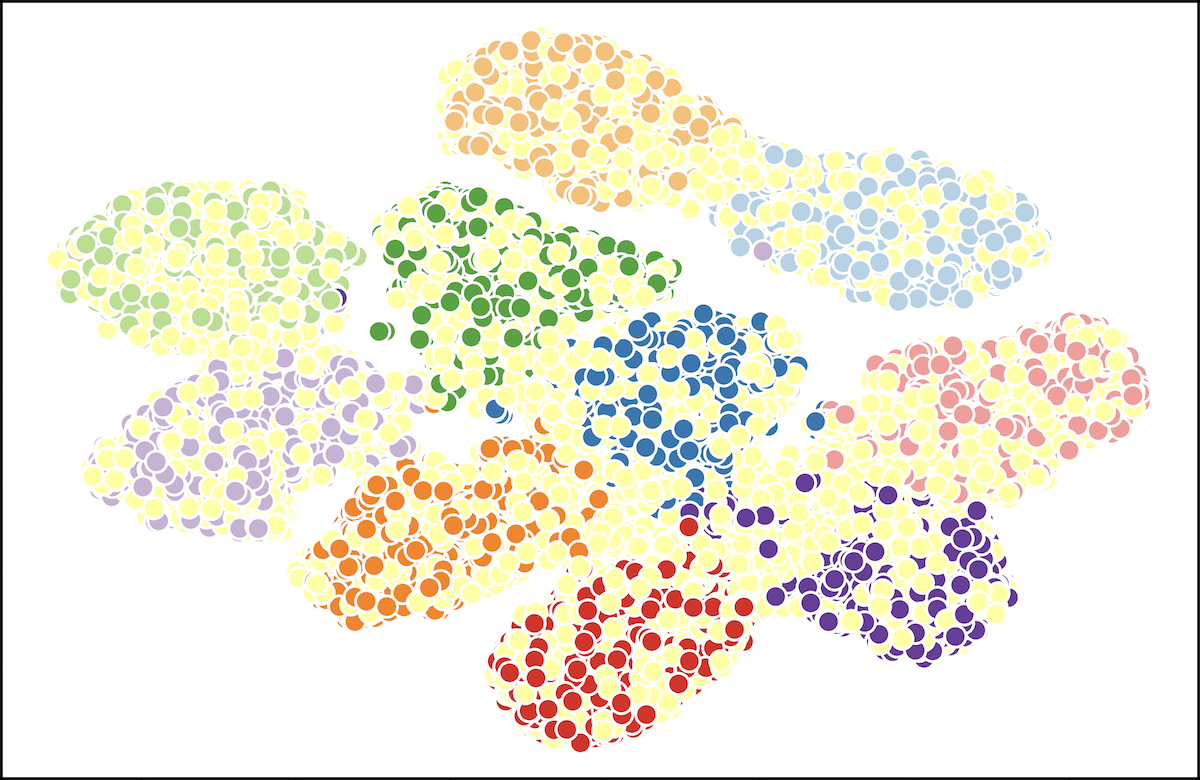
\includegraphics[width=0.32\textwidth]{src/wcl2-cifar10-5.png}}
\caption{WCL tune selection percentage. The first row we use weighted sampling method, the second row we use EGDIS based method.}
\label{Fig.clcifar10}
\end{figure}

In theory, POP tends to select pure boundary samples. EGDIS tends to select samples near two closing clusters and the samples from densest area, which could be anywhere actually. For CL, it tends to select samples far from the boundary, i.e the inner samples. WCL, would choose sample from both the closer cluster boundaries as well as the inner samples. The drawback of CL is that when all the samples are simple enough, with score larger than 0.9, they would tend to act like random selection.



\section{Experiment 3: Logistic Regression Baseline}
We choose 40 and 20 as the number of our extra synthesised datasets, with LR accuracy: 0.78925, 0.853. By fine-tuning the selected subsets, the test accuracy is: 0.8065, 0.8745.

 \begin{figure}[H]
 \centering
 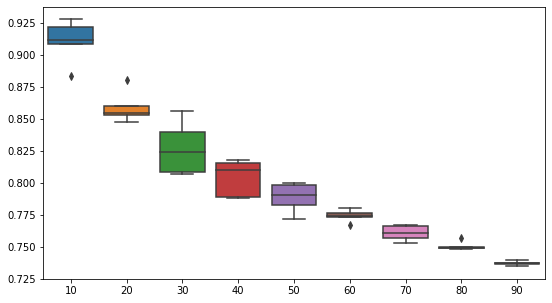
\includegraphics[width=0.8\textwidth]{src/subsets.png}
 \caption{The test set accuracies of CIFAR100 subsets. Horizontal axis is the number of classes selected. Vertical axis is the accuracy score. For each selection, we randomly choose the classes for five times and report the accuracy with logistic regression model.}
 \label{Fig.logistic_subsets}
 \end{figure}
 
 \begin{figure}[H]
\centering  
\subfigure[CIFAR10, 40000 samples]{
\label{Fig.sub.a1}
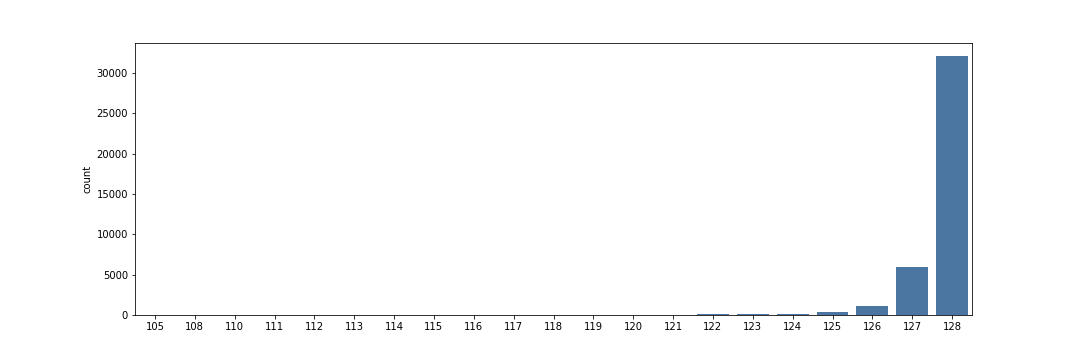
\includegraphics[width=1\textwidth]{src/pop-cifar10-count.png}}
\subfigure[CIFAR20, 8028 samples]{
\label{Fig.sub.a2}
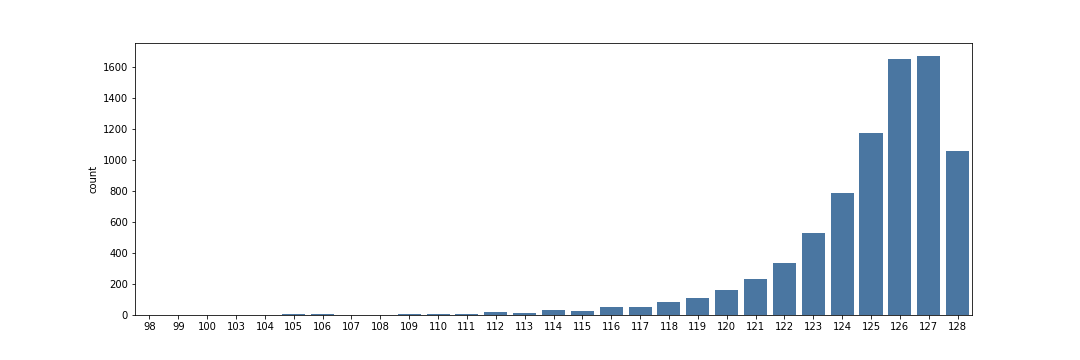
\includegraphics[width=1\textwidth]{src/pop-cifar20-count.png}}
\subfigure[CIFAR40, 16042 samples]{
\label{Fig.sub.a1}
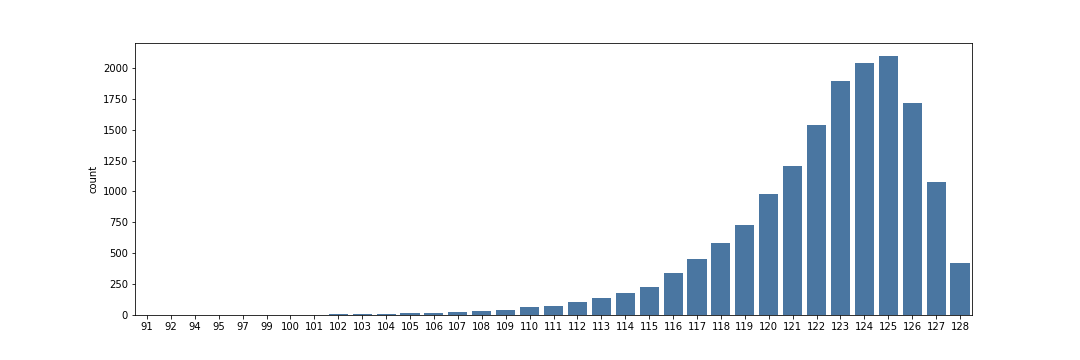
\includegraphics[width=1\textwidth]{src/pop-cifar40-count.png}}
\subfigure[CIFAR100, 40000 samples]{
\label{Fig.sub.a1}
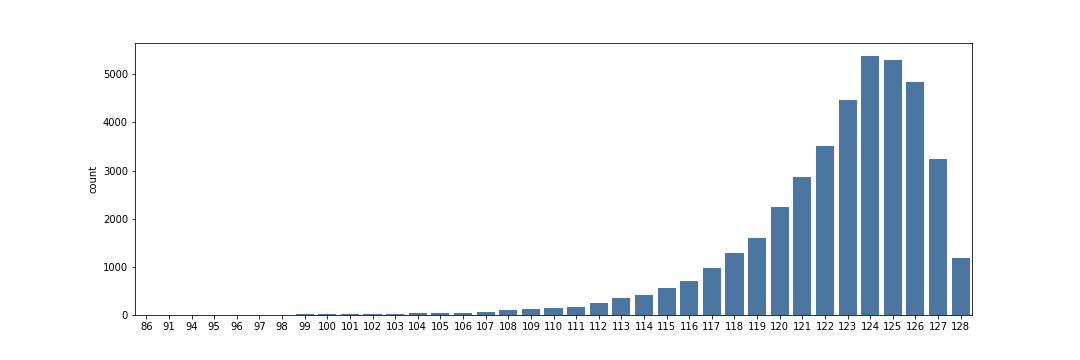
\includegraphics[width=1\textwidth]{src/pop-cifar100-count.png}}
\caption{POP with 4 datasets.}
\label{Fig.clcifar10}
\end{figure}

Even for POP with threshold 1, the number of pure inner is still low. Therefore, it is not good to choose samples with weakness < 128. We fix the number and choose CIFAR samples. From our experiment, we found that the relative accuracy acquired from EGDIS is good enough. Therefore, we make POP to select the same amount of samples as EGDIS, by ranking POP samples based on weakness, to compare their performance.
 
 
 \begin{table}[H]
    \centering
    \begin{tabular}{|l|l|l|l|l|l|l|}
    \hline
        Datasets & NONE & POP & EGDIS & CL & WCL & BWCL \\ \hline
        CIFAR10 & 0.9258 & 0.9258 & \textbf{0.9262} & 0.9234 & 0.9254 & 0.9250 \\ \hline
        CIFAR20 & 0.8825 & \textbf{0.8820} & 0.8738 & 0.8787 & 0.8764 & 0.8775 \\ \hline
        CIFAR40 & 0.8159 & \textbf{0.8130} & 0.8071 & 0.8085 & 0.8115 & 0.8129 \\ \hline
        CIFAR100 & 0.7444 & 0.7398 & 0.7279 & 0.7353 & 0.7404 & \textbf{0.7406} \\ \hline
    \end{tabular}
    \caption{Logistic Regression test set accuracy by averaging 12 runs}
    \label{lgtestacc}
\end{table}

\begin{figure}[H]
\centering  
\subfigure[Relative Accuracy]{
\label{Fig.sub.a1}
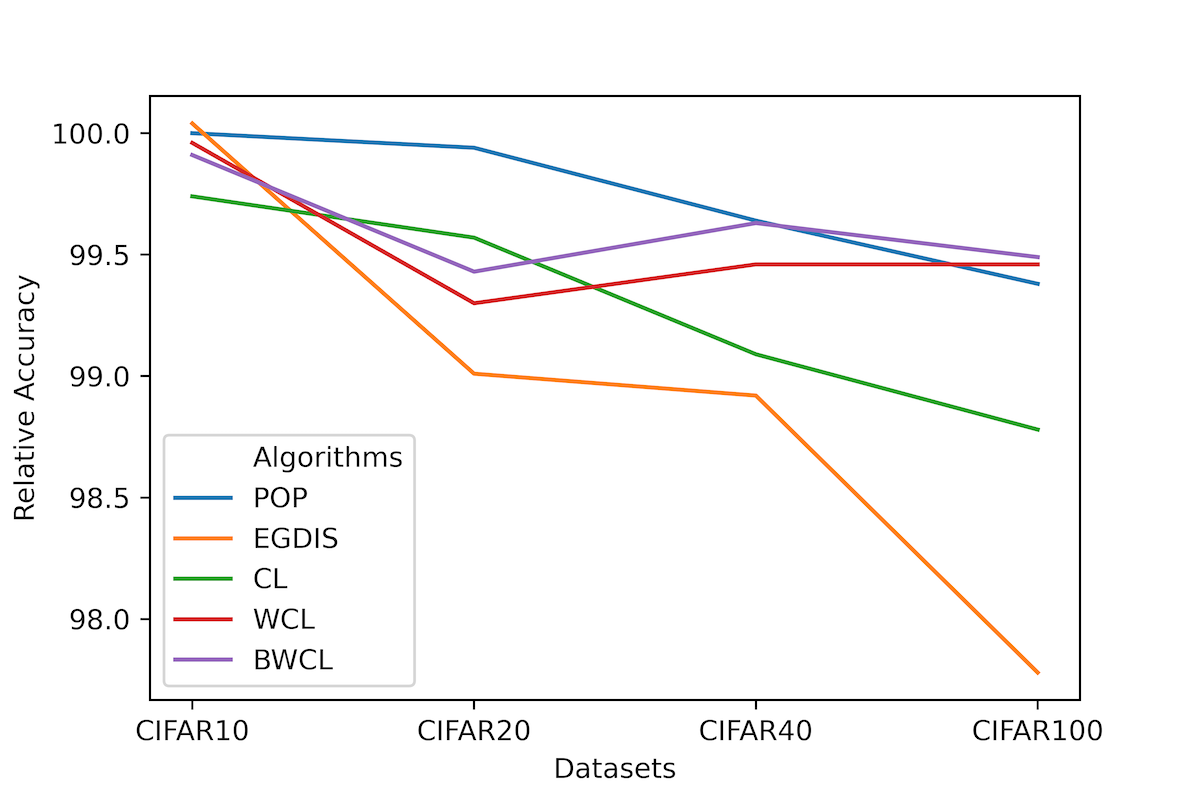
\includegraphics[width=0.45\textwidth]{src/lg_relative.png}}
\subfigure[Relative Accuracy of BWCL by tuning maximum boundary proportion]{
\label{Fig.sub.a2}
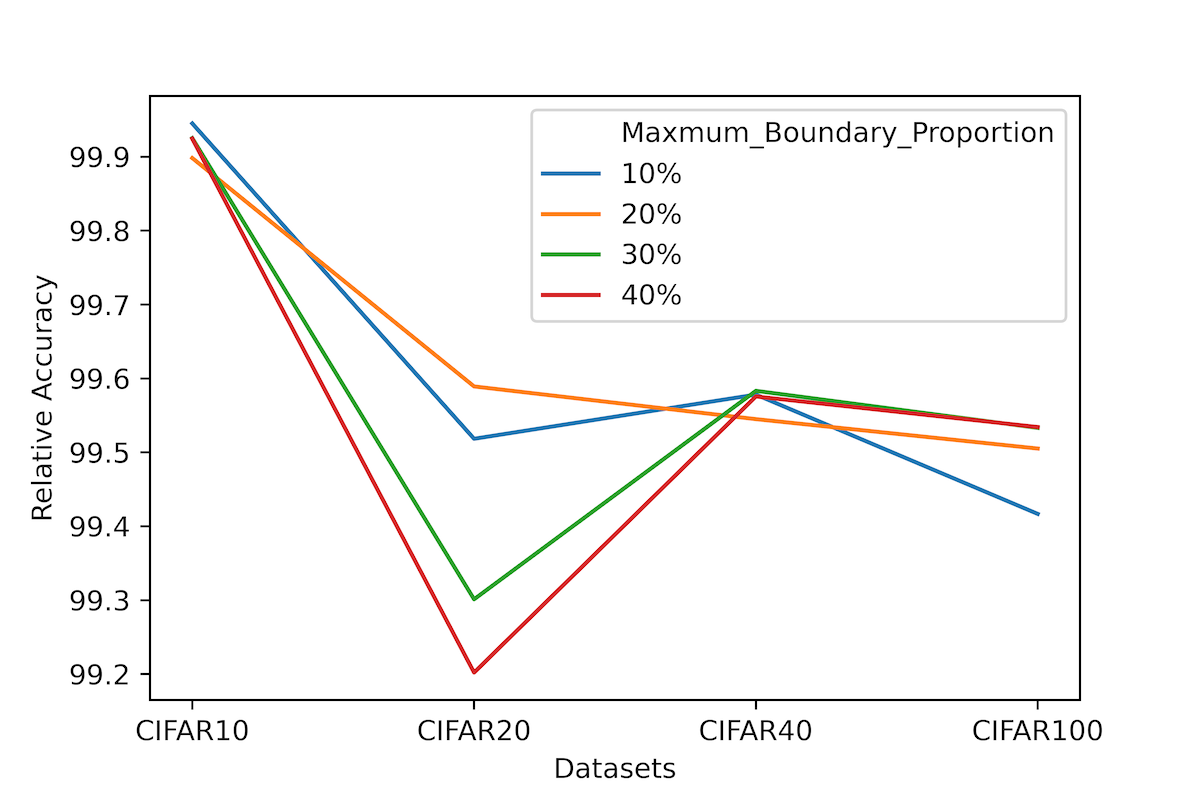
\includegraphics[width=0.45\textwidth]{src/bwcl_relative.png}}
\caption{Relative Accuracy of data reduction algorithms}
\label{Fig.logistic_relativeacc}
\end{figure}

However, this is not a solid conclusion because the quality of the extracted features are so good that the classes are classified easily. We show this effect by varying the proportion of samples selected with BWCL, 0.4.

\begin{figure}[H]
 \centering
 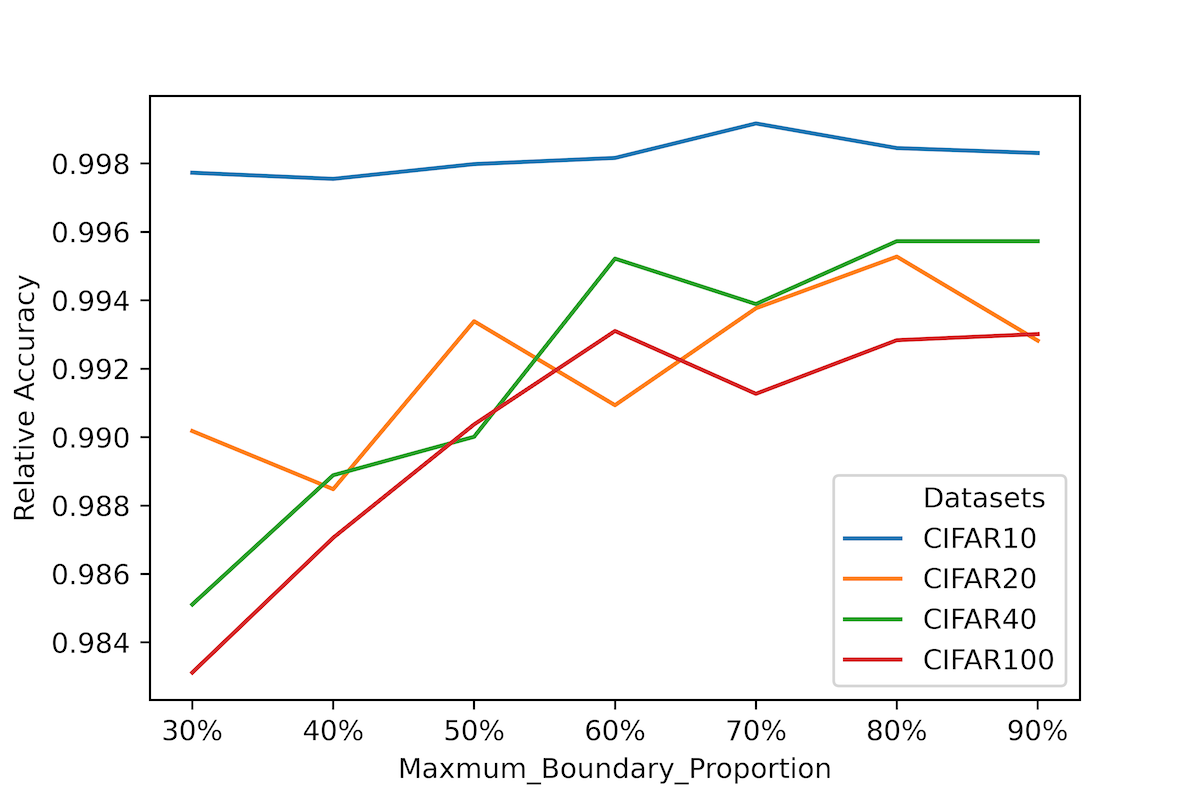
\includegraphics[width=0.8\textwidth]{src/bwcl_relative_size04.png}
 \caption{The test set accuracies of CIFAR100 subsets. Horizontal axis is the number of classes selected. Vertical axis is the accuracy score. For each selection, we randomly choose the classes for five times and report the accuracy with logistic regression model.}
 \label{Fig.logistic_subsets}
 \end{figure}

\subsection{Experiment 4: Data Reduction for CNN}
We train the network densenet101, three times, with learning rate 0.1 (150 epochs), 0.01 (100 epochs) and 0.001 (100 epochs)

\begin{table}[H]
    \centering
    \begin{tabular}{|l|l|l|l|l|l|l|l|}
    \hline
        Datasets & Retention Rate  & NONE & POP & EGDIS & CL & WCL & BWCL \\ \hline
        CIFAR10 & 14.915\% & 95.22 & 82.65 & 81.11 & 82.57 & 84.14 & 81.28 \\ \hline
        CIFAR20 & 16.67\% & 86.6 & 51.9 & 53.2 & 61.45 & 60.05 & 53.1 \\ \hline
        CIFAR40 & 21.09\% & 81.59 & 52.675 & 52.6 & 62.375 & 58.75 & 56.0 \\ \hline
        CIFAR100 & 31.48\% & 78.42 & 59.0 & 57.83 & 64.87 & 65.27 & 64.5 \\ \hline
    \end{tabular}
    \caption{12312312}
    \label{132e3213}
\end{table}


\begin{figure}[H]
\centering  
\subfigure[CIFAR10]{
\label{Fig.sub.a1}
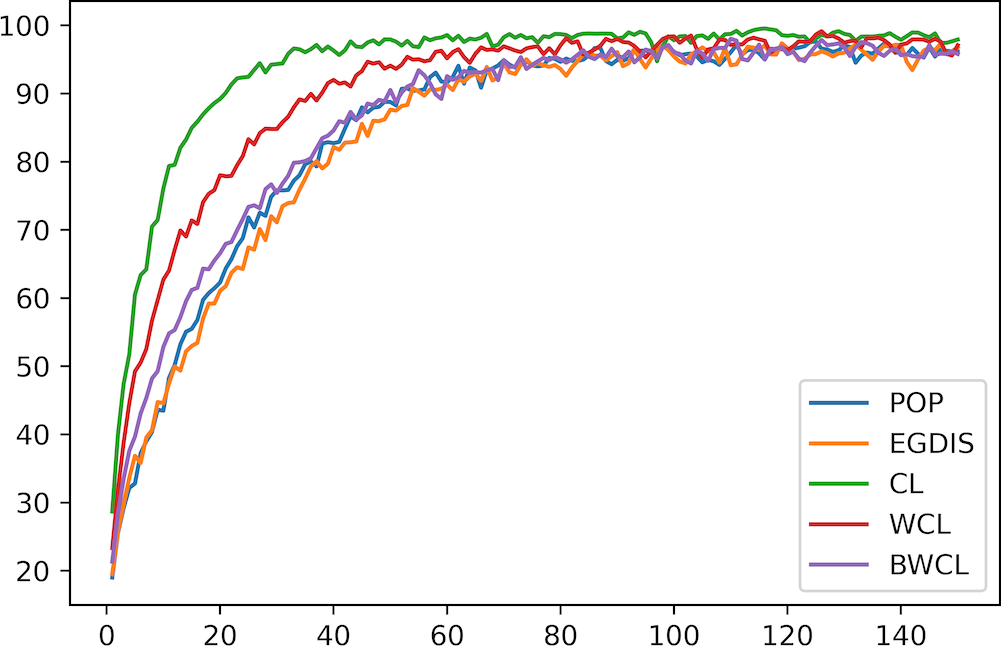
\includegraphics[width=0.45\textwidth]{src/trend_cifar10.png}}
\subfigure[CIFAR100]{
\label{Fig.sub.a2}
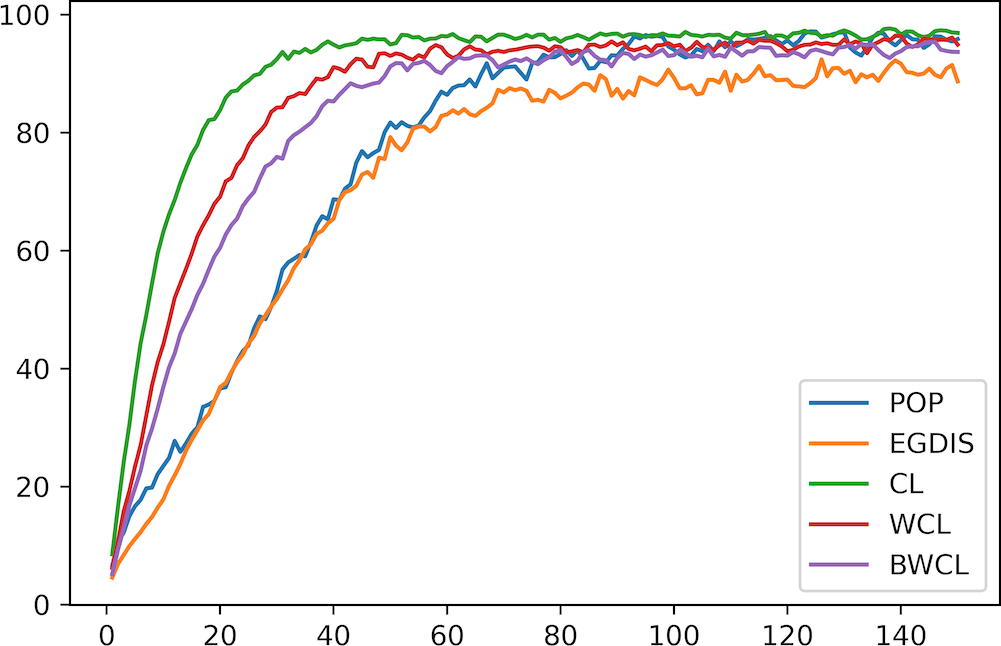
\includegraphics[width=0.45\textwidth]{src/trend_cifar100.png}}

\subfigure[CIFAR20]{
\label{Fig.sub.a2}
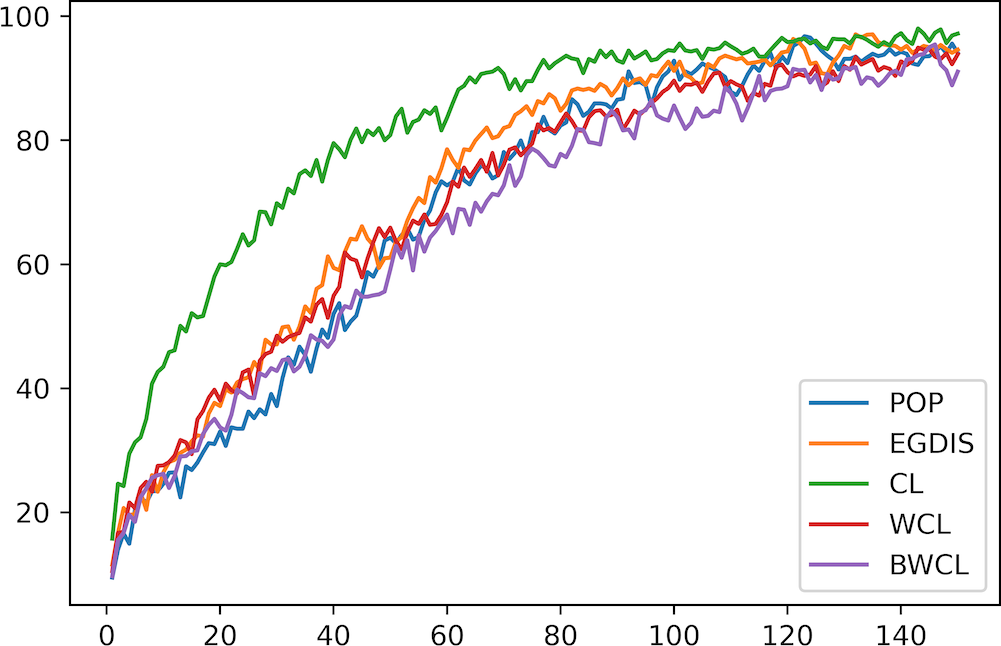
\includegraphics[width=0.45\textwidth]{src/trend_cifar20.png}}
\subfigure[CIFAR40]{
\label{Fig.sub.a2}
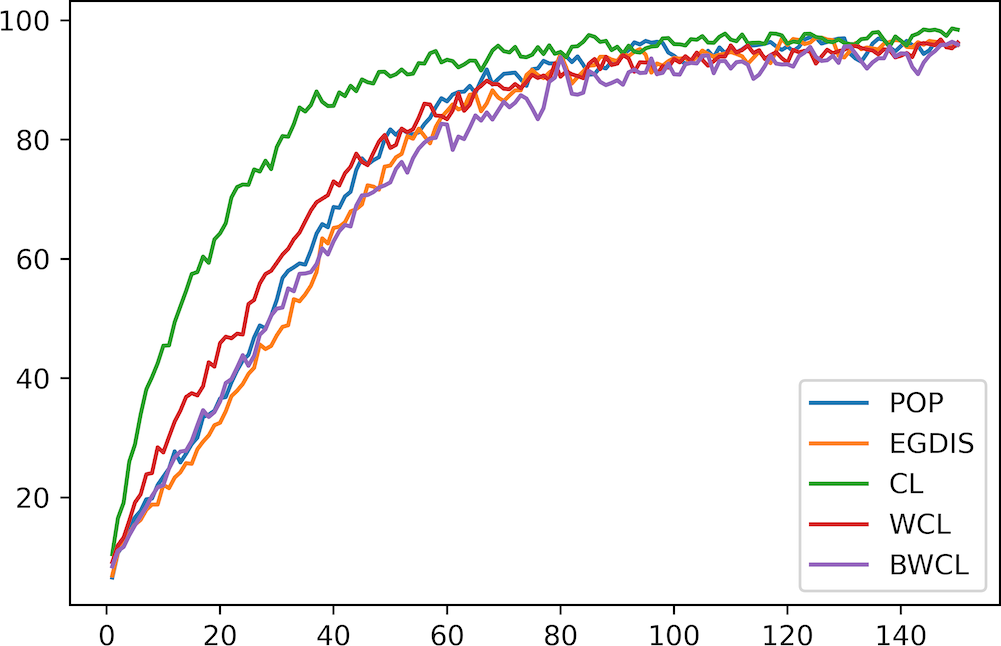
\includegraphics[width=0.45\textwidth]{src/trend_cifar40.png}}
\caption{The training trend of four datasets by selecting the same amount of samples as EGDIS, of the first 150 epochs}
\label{Fig.training_trend}
\end{figure}
